\documentclass[11pt,a4paper,xcolor=dvipsnames]{beamer}
\usetheme{Luebeck}
\usepackage[latin1]{inputenc}
\usepackage[english]{babel}
\usepackage{graphicx}
%\usepackage{qtree}
\usepackage{tikz-qtree}

\usepackage{lmodern}

\author[Michael Cabot \and Sander Latour]{Michael Cabot \and Sander Latour}
\institute{University of Amsterdam}
\title[iMSG]{iterative Minimal Semantics Grammar [iMSG]}

\date{21 maart 2013}

\begin{document}

\begin{frame}
\titlepage
\end{frame}

\begin{frame}
\tableofcontents
\end{frame}

\section{Introduction}
\subsection{Contribution}
\begin{frame}{Contribution}
  \begin{center}
    \textit{How the poverty of the stimulus solves the poverty of the stimulus}\\
    \vfill
    \textbf{combined with}\\
    \vfill
    \textit{The Negotiation and Acquisition of Recursion Grammars as a Result of Competition Among Exemplars}
  \end{center}
\end{frame}

\begin{frame}{Contribution}
  \begin{center}
    \textit{Iteratively evolve a grammar to make it more learnable}\\
    \vfill
    \textbf{combined with}\\
    \vfill
    \textit{Learning a semantic grammar from observations}
  \end{center}
\end{frame}

\begin{frame}{Contribution}
  \begin{center}
    \textit{Iteratively evolve a grammar to make it more learnable}\\
    \vfill
    \textbf{Iteratively evolve a semantic grammar}\\
    \vfill
    \textit{Learning a semantic grammar from observations}
  \end{center}
\end{frame}

\subsection{Motivation}
\begin{frame}{Motivation}
  \begin{itemize}
    \item \hspace*{0pt}[Zuidema2003] needed to force minimal language size
    \item Language is driven by the need to communicate semantic messages
    \item The necessity to be able to communicate may make forcing obsolete
    \item The negotiation model of [Batali1999] seems convertable to the iterative process of evolution
  \end{itemize}
\end{frame}

\subsection{Background}
\begin{frame}{Iterative Learning}
  \begin{center}
    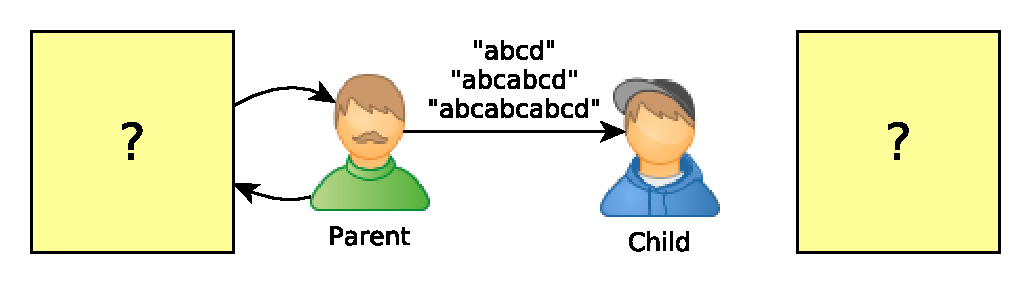
\includegraphics[scale=0.6]{assets/iterative1.pdf}
  \end{center}
\end{frame}

\begin{frame}{Iterative Learning}
  \begin{center}
    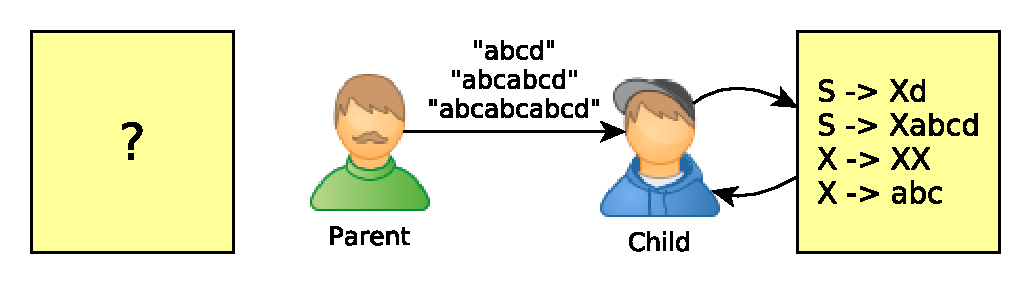
\includegraphics[scale=0.6]{assets/iterative2.pdf}
  \end{center}
\end{frame}

\begin{frame}{Iterative Learning}
  \begin{center}
    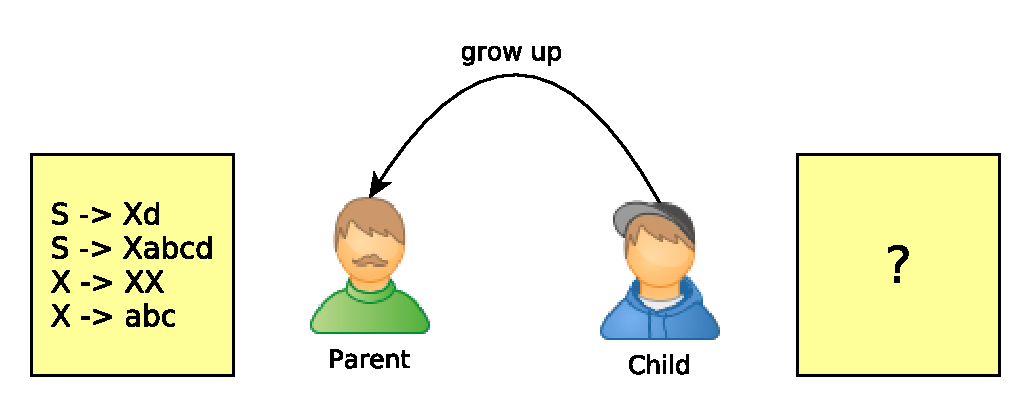
\includegraphics[scale=0.6]{assets/iterative3.pdf}
  \end{center}
\end{frame}

\begin{frame}{Semantic vocabulair}
  \begin{columns}[c]
    \column{.65\textwidth}
      \begin{description}
        \item[meaning] set of predicates and relations
        \item[sentence] concatenated strings (i.e. words)
        \item[observation] Alignment of meaning and sentence
        \item[phrase] Hierarchical structure from meaning to string
        \item[examplar phrase] Lexicon
        \item[complex phrase] Conjunction of two phrases
      \end{description}
    \column{.35\textwidth}
      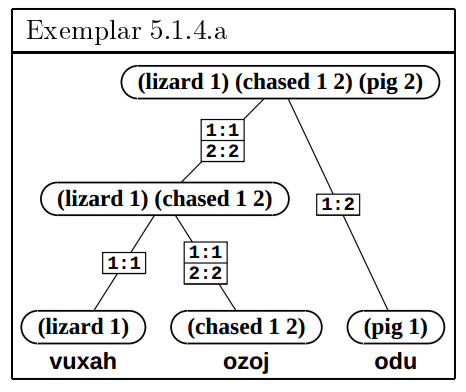
\includegraphics[scale=0.2]{assets/examplar514a.png}
  \end{columns}
  \hfill 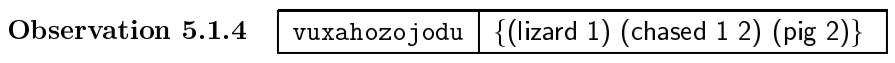
\includegraphics[scale=0.2]{assets/observation514.png}
\end{frame}

\begin{frame}{Batali}
  \begin{itemize}
    \item Simplified support for grammar and semantics
    \item Inducing phrases by creation or alteration
    \item Phrases have costs based on their construction
    \item Encourage and discourage to update ``probabilistic'' model
  \end{itemize}
\end{frame}

\section{iMSG}
\subsection{Assumptions}
\begin{frame}{Assumptions}
\begin{itemize}
  \item The sentence is separated in words (vs. one signal)
  \item The order in the meaning corresponds to the order of the words
  \item Words are first encountered separately before used in sentences
\end{itemize}
\end{frame}

\begin{frame}
  \begin{center}
  {\Huge \textbf{Iteratively evolve a semantic grammar}}
  \end{center}
\end{frame}

\subsection{Generating observations}%(Michael)

\begin{frame}{Introducing templates}
\begin{itemize}
  \item Template set: $\langle$[P(1)], ..., [P(1),R(1,2),P(2)], ...$\rangle$
  \item Formula pools:
  \begin{itemize}
    \item predicates: [snake, pig, ..., walks, smiles, ...] % nouns and intransitive verbs
    \item relations: [loves, bites, ...] % transitive verbs
  \end{itemize}
  \item Probability distribution based on exemplar costs
\end{itemize}
\end{frame}

\begin{frame}{Generating meaning}
\begin{itemize}
  \item Take template. E.g. \textit{ Predicate(1) Relation(1,2) Predicate(2) }
  \item For each placeholders in template:
  \begin{itemize}
    \item Sample formula from formula pool
  \end{itemize}
  \item E.g: \textit{ snake(1) bites(1,2) pig(2) }
\end{itemize}
\end{frame}

\begin{frame}{Generating sentence}
\begin{itemize}
  \item Given meaning and PCFG: generate sentence (top-down)
\end{itemize}
\end{frame}

\subsection{ViterbiX} %(Michael)
\begin{frame}{ViterbiX (Viterbi eXtended)}
\begin{itemize}
  \item Expand nodes X,Y in adjacent spans in chart with:
  \begin{itemize}
    \item $A \rightarrow B,C$, where $B \subseteq X$ and $C \subseteq Y$
    \item $M(X \cup Y) \rightarrow X,Y$
    \item Note: for all possible argument mappings
  \end{itemize}
\end{itemize}
\end{frame}

\begin{frame}{Example}
Substitution:\\
\begin{figure}[!h]
\centering
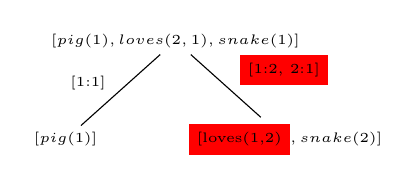
\begin{tikzpicture}[
   level distance=1.25cm,sibling distance=1cm,
   edge from parent path={(\tikzparentnode) -- (\tikzchildnode)}]
\tiny
\Tree
[.\text{$[pig(1), loves(2,1), snake(1)]$}
    \edge node[auto=right,pos=.6] {[1:1]};
    [.\text{$[pig(1)]$}
        ]
    \edge node[auto=left,pos=.6] {\colorbox{red}{[1:2, 2:1]}};
    [.\text{$\colorbox{red}{[loves(1,2)}, snake(2)]$} 
        ]
]
\end{tikzpicture}
$\rightarrow$
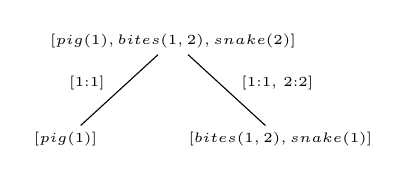
\begin{tikzpicture}[
   level distance=1.25cm,sibling distance=1cm,
   edge from parent path={(\tikzparentnode) -- (\tikzchildnode)}]
\tiny
\Tree
[.\text{$[pig(1), bites(1,2), snake(2)]$}
    \edge node[auto=right,pos=.6] {[1:1]};
    [.\text{$[pig(1)]$}
        ]
    \edge node[auto=left,pos=.6] {[1:1, 2:2]};
    [.\text{$[bites(1,2), snake(1)]$} 
        ]
]
\end{tikzpicture}
\end{figure}

\end{frame}

\subsection{Learning}
\begin{frame} %(Michael)
\frametitle{Learning from observations using ViterbiX}
\begin{description}
  \item[$T$] ViterbiX parses for sentence
  \item[$\tau_o \in T$] Parse with meaning of observation
  \item[$c(\tau)$] cost of ViterbiX parse
  \item[$T_s \subset T$] all parses with lower cost than $c(\tau_o)$
\end{description}

\begin{itemize}
\item For every rule in $\tau_o$:
    \begin{itemize}
      \item Reinforce rule
    \end{itemize}
  \item For every $\tau_s$ in $T_s$:
    \begin{itemize}
      \item For every rule in $\tau_s$:
        \begin{itemize}
          \item Discourage rule
        \end{itemize}
    \end{itemize}
\end{itemize}
\end{frame}

\section{Evaluation}
\begin{frame}{Evaluation} %(Michael)
\begin{itemize}
  \item Grammar size
  \item Verbalization costs
  \item Parse costs
  \item Cost difference between $T_s$ and $\tau_o$
\end{itemize}
\end{frame}

\section{Status} % (Sander)
\begin{frame}{Current Status}
  \begin{itemize}
    \item Largely implemented [Batali1999] learning algorithm with iterations
    \item Iterative development process $\Rightarrow$ redesign
    \item Implementation as presented will be finished and evaluated
  \end{itemize}
\end{frame}

\begin{frame}{Questions?}
  \begin{center}
  {\Large $\exists x \left[ question(x) \land \neg covered(x) \right]$?}
\end{center}
\end{frame}
\end{document}
